\documentclass{beamer}
\usetheme{Madrid}
\usepackage{amsfonts}
\usepackage{graphicx}
\usepackage{amsmath, amssymb, amsthm}
\usepackage{graphicx}
\usepackage{listings}
\usepackage{gensymb}
\usepackage[utf8]{inputenc}
\usepackage{hyperref}
\usepackage{gvv}
\usepackage{tikz}
\usepackage{minted}

\usetikzlibrary{decorations.pathmorphing}

\begin{document}
\title{MATGEO - 7-7.2-22}
\author{AI24BTECH11008 - G. Sarvajith}
\date{\today}
\frame{\titlepage}

\begin{frame}{Question}
    Find the equation of the circle having (1, -2) as its centre and passing through the
    intersection of $3x + y = 14, 2x + 5y = 18$.
\end{frame}

\begin{frame}{allowframebreaks}
\frametitle{Terms Used}
\begin{table}[htbp]
    \centering
    \caption{Terms used}
    \label{tab:parameters}
    \begin{tabular}{|p{1.7cm}|p{4cm}|}
        \hline
        \textbf{varaibles} & \textbf{values}\\
        \hline
        \textbf{centre} & $\myvec{1\\-2}$\\
        \hline
        \textbf{line 1} & $3x + y = 14$\\
        \hline
        \textbf{line 2} & $2x + 5y = 18$\\
        \hline
    \end{tabular}
\end{table}
\end{frame}
\begin{frame}{Solution}
    Intersection point of the 2 linear equations $3x + y = 14$ and $2x + 5y = 18$ is given by\\
    \begin{align*}
    \myvec{3 & 1\\2 & 5}\myvec{x \\ y} = \myvec{14\\18}\\
    \end{align*}  
\end{frame}
\begin{frame}{Row Reduction}
    \begin{align*}
        \begin{bmatrix}3 & 1 & 14\\2 & 5 & 18\end{bmatrix}\longleftrightarrow[{R_2 \leftarrow {3R_2-2R_1}}]\begin{bmatrix}3 & 1 & 14\\0 & 13 & 26\end{bmatrix}\\
        \longleftrightarrow[{R_2 \leftarrow {R_2/13}}]\begin{bmatrix}3 & 1 & 14\\0 & 1 & 2\end{bmatrix}\\
        \longleftrightarrow[{R_1 \leftarrow {R_1-R_2}}]\begin{bmatrix}3 & 0 & 12 \\0 & 1 & 2\end{bmatrix}\\
        \longleftrightarrow[{R_1 \leftarrow {R_1/3}}]\begin{bmatrix}1& 0 & 4\\0 & 1 & 2\end{bmatrix}\\
        \end{align*}
        $\therefore$ the intersecting point of the 2 lines is A(4,2).
\end{frame}
\begin{frame}{Solution}
    \begin{align*}
        r = \norm{A-C} = \sqrt{\brak{A-C}^T\brak{A-C}} 
    \end{align*}
    Where A\brak{4,2} is point of intersection and point on the circle with the centre C\brak{1,-2}.
    \begin{align*}
        r = \sqrt{\myvec{3 & 4}\myvec{3\\4}} = 5
    \end{align*}
    equation of a conic is given by  $x^TVx + 2u^Tx + f = 0$\\
     for a circle
    \begin{align*}
     V &= \myvec{1&0\\0&1},\\ 
    u&=\myvec{-h\\-k}, \\
    f &= \norm{u}^2 - r^2\\
    \end{align*}
\end{frame}
    \begin{frame}
        substituting the above values in the equation we get 
    \begin{align*}
    x^Tx + 2\myvec{-1 & 2}x - 20 = 0
    \end{align*}
    \end{frame}
    
 
\begin{frame}[fragile,allowframebreaks]
\frametitle{C code for finding }
\begin{minted}[linenos=true]{c}
    #include <stdio.h>

    void sol(int m, int a[m], int b[m], int x[m-1]){
        int p,q;
        p = (a[1]*b[2]-a[2]*b[1])/(a[0]*b[1]-a[1]*b[0]);
        q = (a[2]*b[0] - a[0]*b[2])/(a[0]*b[1] - a[1]*b[0]);
        x[0] = p;
        x[1] = q;
    }
    \end{minted}
\end{frame}
\begin{frame}[fragile, allowframebreaks]
    \frametitle{Python code for graph}
    \begin{standalone}
        \begin{minted}[fontsize=\tiny, linenos=true]{python}
        import ctypes
import numpy as np
import matplotlib.pyplot as plt
# Load the shared library
solution_lib = ctypes.CDLL('./libsolution.so')

# Set the argument types for the 'sol' function

solution_lib.sol.argtypes = 
[ctypes.c_int, ctypes.POINTER(ctypes.c_int),ctypes.POINTER(ctypes.c_int), ctypes.POINTER(ctypes.c_int)]

# Define input arrays
m = 3
a = (ctypes.c_int * m)(3, 1, -14)  # int a[3] = {3, 1, -14}
b = (ctypes.c_int * m)(2, 5, -18)  # int b[3] = {2, 5, -18}
x = (ctypes.c_int * (m - 1))()  # int x[2];
        \end{minted}
    \end{standalone}
    \end{frame}

\begin{frame}[fragile, allowframebreaks]
    \scriptsize
    \frametitle{Python code for graph}
    \begin{minted}[linenos=true]{python}
# Call the C function
solution_lib.sol(m, a, b, x)

# Retrieve the point from x array
point_x = x[0]
point_y = x[1]

# Print the point
print(f"Point on the circle: ({point_x}, {point_y})")
# Define the center of the circle
center = (1, -2)
# Calculate the radius
radius = np.sqrt((point_x - center[0])**2 +              (point_y - center[1])**2)
 \end{minted}
\end{frame}
\begin{frame}[fragile, allowframebreaks]
    \scriptsize
    \frametitle{Python code for graph}
    \begin{minted}[linenos=true]{python}
# Create circle data with more points
theta = np.linspace(0, 2 * np.pi, 1000) 
circle_x = center[0] + radius * np.cos(theta)
circle_y = center[1] + radius * np.sin(theta)

# Create line data for 3x + y = 14
x_line1 = np.linspace(center[0] - radius - 2,center[0] + radius + 2, 100)
y_line1 = 14 - 3 * x_line1  # Rearranged: y = 14 - 3x

# Create line data for 2x + 5y = 18
x_line2 = np.linspace(center[0] - radius - 2, center[0] + radius + 2, 100)
y_line2 = (18 - 2 * x_line2) / 5  # Rearranged: y = (18 - 2x) / 5

# Plot the circle and lines
plt.figure(figsize=(8, 8))
plt.plot(circle_x, circle_y, label='Circle', color='blue')
\end{minted}
\end{frame}
\begin{frame}[fragile, allowframebreaks]
    \scriptsize
    \frametitle{Python code for graph}
\begin{minted}[fontsize=\tiny,linenos=true]{python}
plt.plot(x_line1, y_line1,label='Line: 3x + y = 14',color='orange')
plt.plot(x_line2, y_line2, label='Line: 2x + 5y = 18',color='purple')
plt.scatter(*center, color='red', label='Center (1, -2)')
plt.scatter(point_x,point_y,color='green', label=f'Point ({point_x}, {point_y})')

# Set appropriate limits for better view
plt.xlim(center[0]-radius-2,center[0]+radius+2)
plt.ylim(center[1]-radius-2,center[1]+radius+2)

plt.axhline(0,color='black',linewidth=0.5,ls='--')
plt.axvline(0,color='black',linewidth=0.5,ls='--')
plt.grid()
plt.gca().set_aspect('equal', adjustable='box') 
plt.title()('Circle with Center (1, -2),Point from C Code, and Lines')
plt.legend()
plt.show()
\end{minted}
\end{frame}
\begin{frame}{Figure}
    \begin{center}
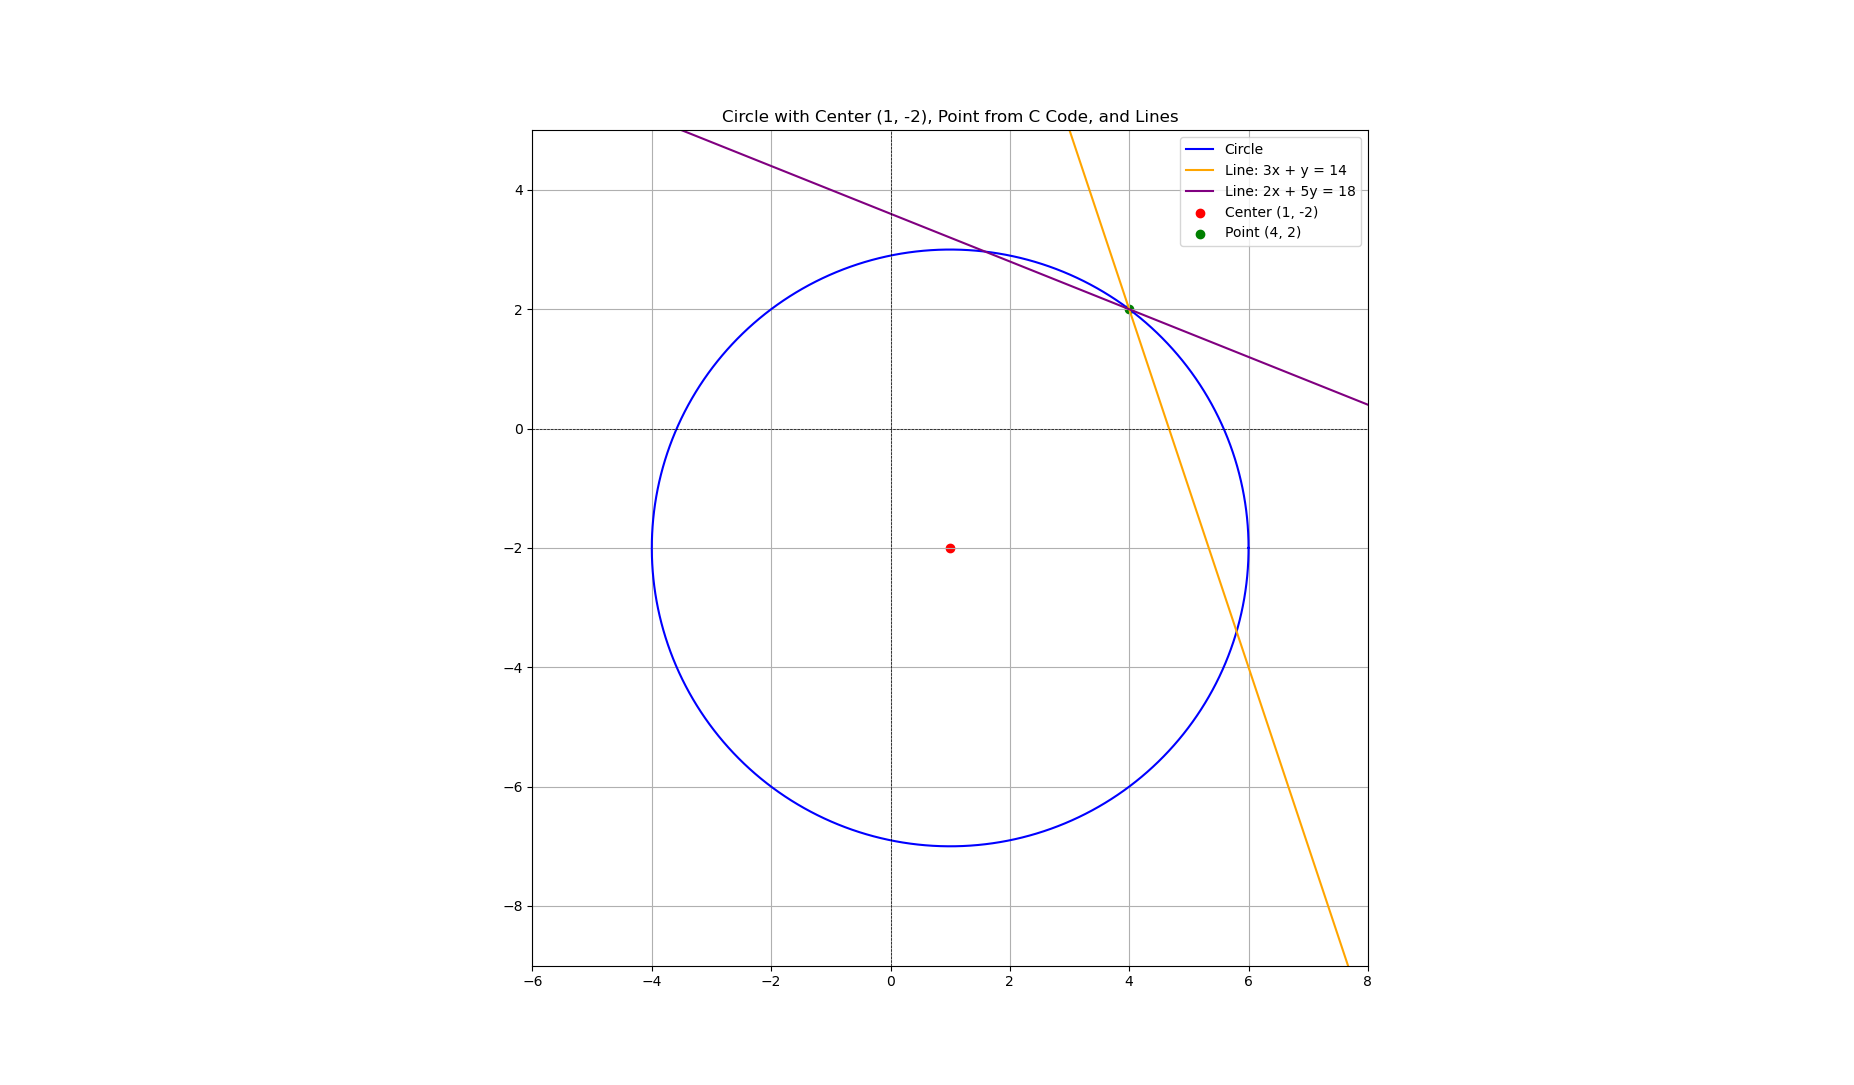
\includegraphics[width=0.9\textwidth]{figs/Figure_1.png}
\end{center}
\end{frame}
\end{document}